\chapter{Evaluation}
\label{sec:eval} 

\begin{figure}[H]
    \hspace*{-2.5cm}
    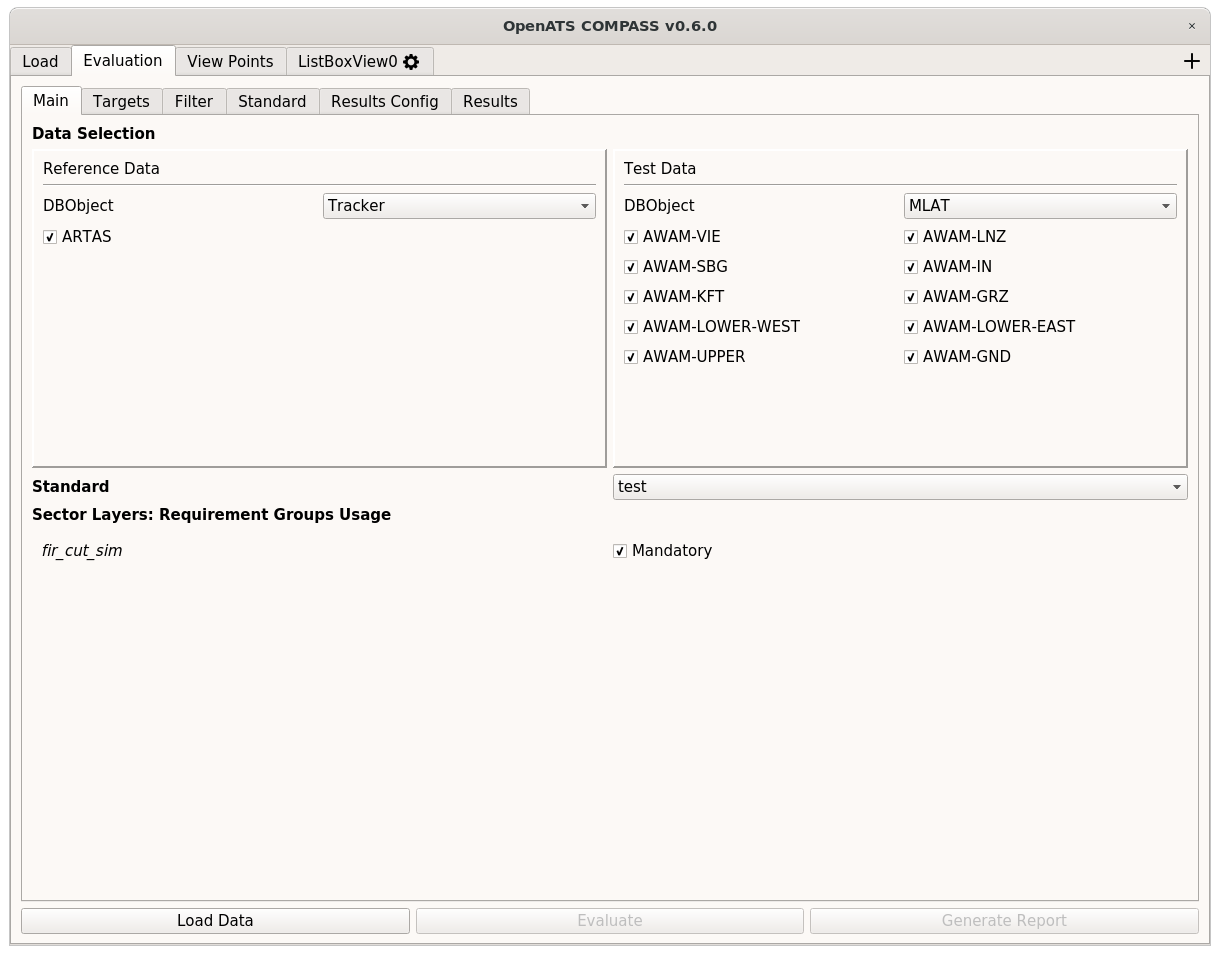
\includegraphics[width=19cm]{figures/eval.png}
  \caption{Evaluation tab}
\end{figure}

The 'Evaluation' tab allows adapting/defining requirement-based standards  and compliance assessment of said standards. \\

Please \textbf{note} . \\

\section{Pre-Requisites \& Limitations}
\label{sec:eval_prereq} 

\begin{itemize}  
\item Target report associations must be set (using \nameref{sec:task_associate_tr})
\item At least 1 sector has to be defined (using \nameref{sec:task_manage_sectors})
\item Usable reference data must exist
\item Usable test data must exist
\end{itemize}
\ \\

While it is possible to manually remove single targets from the evaluation, the usage of correct reference data is paramount for the significance of the evaluation results. \\

\includegraphics[width=0.5cm]{../../data/icons/hint.png} \textbf{Please note that the evaluation feature is currently being tested/verified and should be used for such purposes only. It should not be used as a sole basis for decision making - especially not without manually verifying the evaluation results.} \\

There will be improvements in the next releases, and further verification of the results by the author and other users.

\subsection{Target Report Associations}

Since the task only makes use of the Mode S address, non-Mode S data is not evaluated and may even show up as gaps/misses in detection.

\subsection{Sector Altitude Filtering}

If sectors with altitude limits are used, please be aware that target reports without a Mode C code can not be filtered by the set limit. Therefore such target reports are assumed to be inside in all sectors when inside the defined 2D polygons. \\

The 'inside-sector' check is always performed on the reference data only, therefore it is of importance to only use reference data with existing Mode C code data.

\subsection{Reference Data}

The assumption used in the tool is that the reference data is always correct. Therefore, sub-optimal reference data can cause errors, which will be attributed to the test data in the evaluation. \\

To give a few examples what this could mean:
\begin{itemize}  
\item Wrong 'inside-sector' check results: This might remove valid test data from the evaluation and/or attribute errors to the wrong sector
\item Missing target data in reference: This will remove the test data from evaluation for the time-period of the missing reference data
\item Wrong position in reference: This will cause wrong 'inside-sector' check results and/or cause wrong horizontal position accuracy results
\item Wrong/missing Mode C code in reference: This will cause wrong 'inside-sector' check results
\item Wrong/missing identification in reference: This will cause wrong results in identification requirements
\end{itemize}
\ \\

Also, since target secondary attributes (currently only Mode S address) are also used in the 'Target Report Association' task, errors in these attributes might also lead to imperfect data association. This would result in wrong evaluation results in almost all requirements.

\section{Overview}
\label{sec:eval_overview} 

\begin{figure}[H]
  \hspace*{-2cm}
    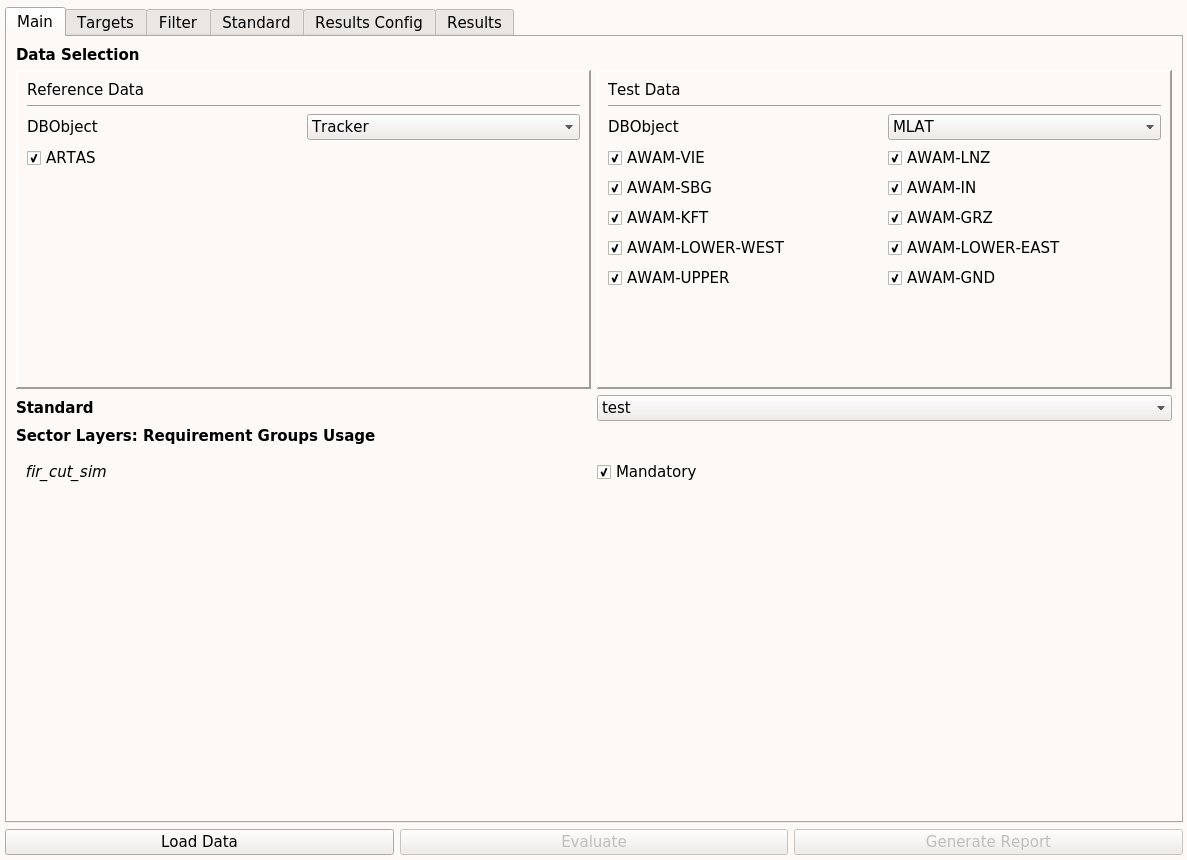
\includegraphics[width=18cm,frame]{figures/eval_overview.png}
  \caption{Evaluation overview}
\end{figure}

At the top, 6 tabs exist:
\begin{itemize}  
\item Main: Main configuration
\item Targets: Table of existing targets (filled after data was loaded)
\item Filter: Filter which data is loaded, by time and/or ADS-B quality indicators
\item Standard: Definition of standards, selection of current standard, configuration of requirements to be checked
\item Results Config: Additional configration for the result generation
\item Results: Evaluation results (created after data was evaluated)
\end{itemize}
\ \\

Below 3 buttons exist:
\begin{itemize}  
\item Load Data: Loads the reference/test data
\item Evaluate: Runs the evaluation of the current standard (available after data was loaded)
\item Generate Report: Generates a report PDF (available when evaluation result exists)
\end{itemize}
\ \\

\section{Configuration}
\label{sec:eval_config} 

\subsection{Main Tab}

\begin{figure}[H]
  \hspace*{-2cm}
    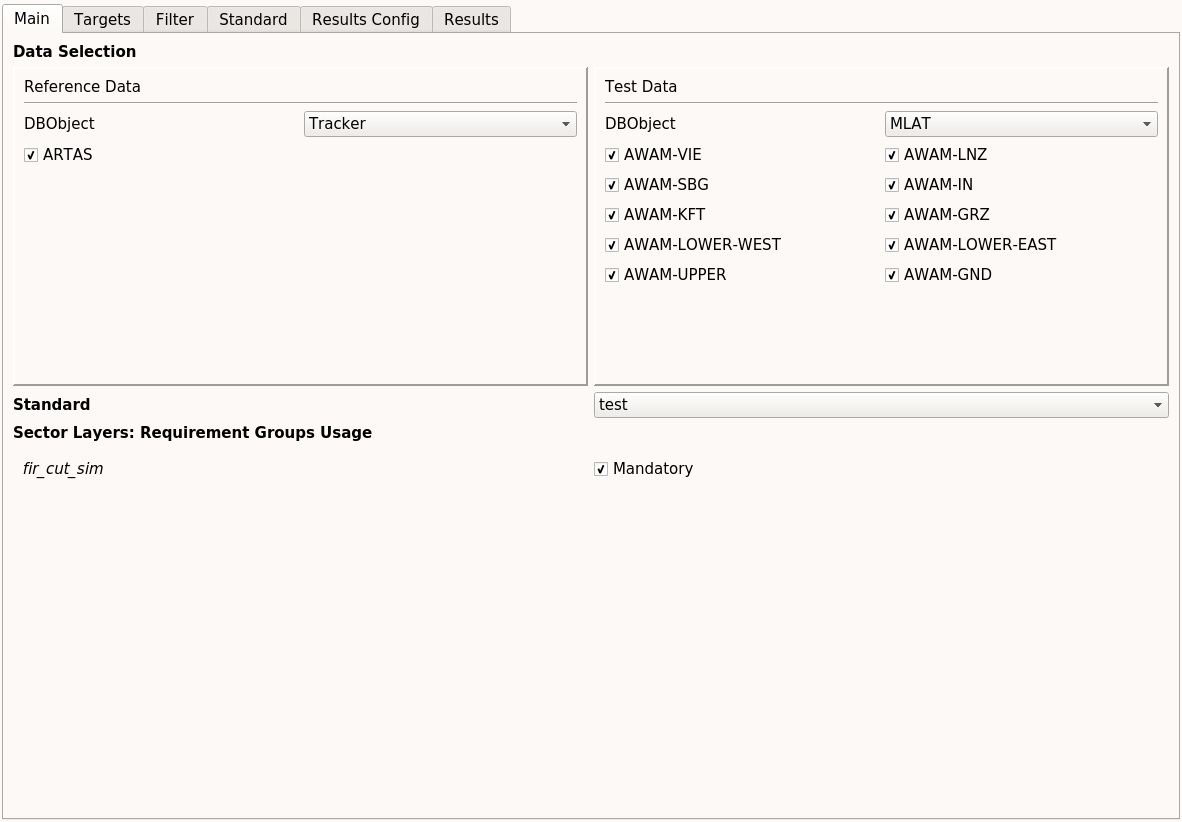
\includegraphics[width=18cm,frame]{figures/eval_main.png}
  \caption{Evaluation Main tab}
\end{figure}

In the main tab, the main configuration settings can be set. \\

\subsubsection{Data Selection}

At the top, the 'Data Selection' can be performed, by selecting:
\begin{itemize}  
\item Reference Data:
\begin{itemize}  
\item DBObject: Any DBObject existing in the database
\item Data source checkboxes: Which data sources to use
\end{itemize}
\item Test Data:
\begin{itemize}  
\item DBObject: Any DBObject existing in the database
\item Data source checkboxes: Which data sources to use
\end{itemize}
\end{itemize}
\ \\

As noted before, usage of appropriate reference data is of paramount importance. \\

Since 'any' type of data can be selected for evaluation, this allows for the following use-cases:
\begin{itemize}  
\item Tracker as reference, sensor as test data: Evaluation of sensor
\item Tracker as reference, tracker as test data: Evaluation/comparison of different trackers/tracker runs
\end{itemize}
\ \\

Of course it is also possible to use e.g. an imported GPS trail as reference (see \nameref{sec:task_import_gps}), although this is currently not tested for lack of test data. If you might be able to provide such test data, please contact the author. \\

\subsubsection{Standard}
In the center, using the 'Standard' drop-down menu, the current standard can be selected. To create/configure the standard please use the 'Standard' tab.

\subsubsection{Sector Layer/Requirement Mapping}

Below that, the 'Sector Layers: Requirement Groups Usage' allows to define which requirements should be verified for which sector layer. \\

On the left, all existing sector layers are listed, in the shown example:
\begin{itemize}  
\item fir\_cut\_sim: DOI altitude limitation
\end{itemize}
\ \\

For each sector layer, the requirement groups (defined in the Standard tab) can be active/disabled. In the shown example, the existing requirement group 'Mandatory' is active in the sector layer.

\subsection{Targets Tab}

\begin{figure}[H]
  \hspace*{-2cm}
    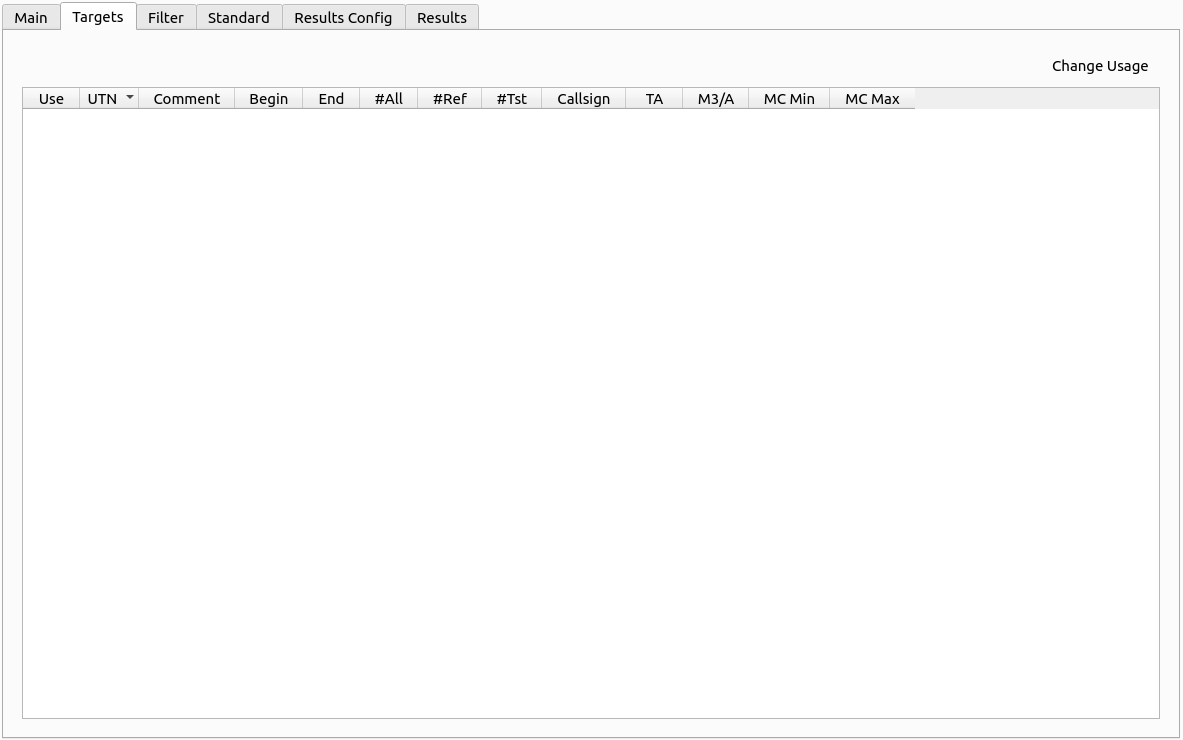
\includegraphics[width=18cm,frame]{figures/eval_targets_empty.png}
  \caption{Evaluation Targets tab}
\end{figure}

Before the data was loaded, the table is empty. Each target (defined by the UTN) is shown in a dedicated row. \\

The following columns exist:

\begin{itemize}  
\item Use: Checkbox defining if the target should be used in the evaluation
\item UTN: Unique Target Number
\item Begin: First timestamp of UTN
\item End: Last timestamp of UTN
\item \#All: Sum number of target reports
\item \#Ref: Number of target reports in reference data
\item \#Tst: Number of target reports in test data
\item Callsign: Target identification(s)
\item TA: Target address (hexadecimal)
\item M3/A: Mode 3/A code(s) (octal)
\item MC Min: Mode C code minimum [ft]
\item MC Max: Mode C code maximum [ft]
\end{itemize}
\ \\

Unless otherwise specified, the column content reflects the values from both reference and test data. \\

After loading the data, the table can look as follows:

\begin{figure}[H]
  \hspace*{-2cm}
    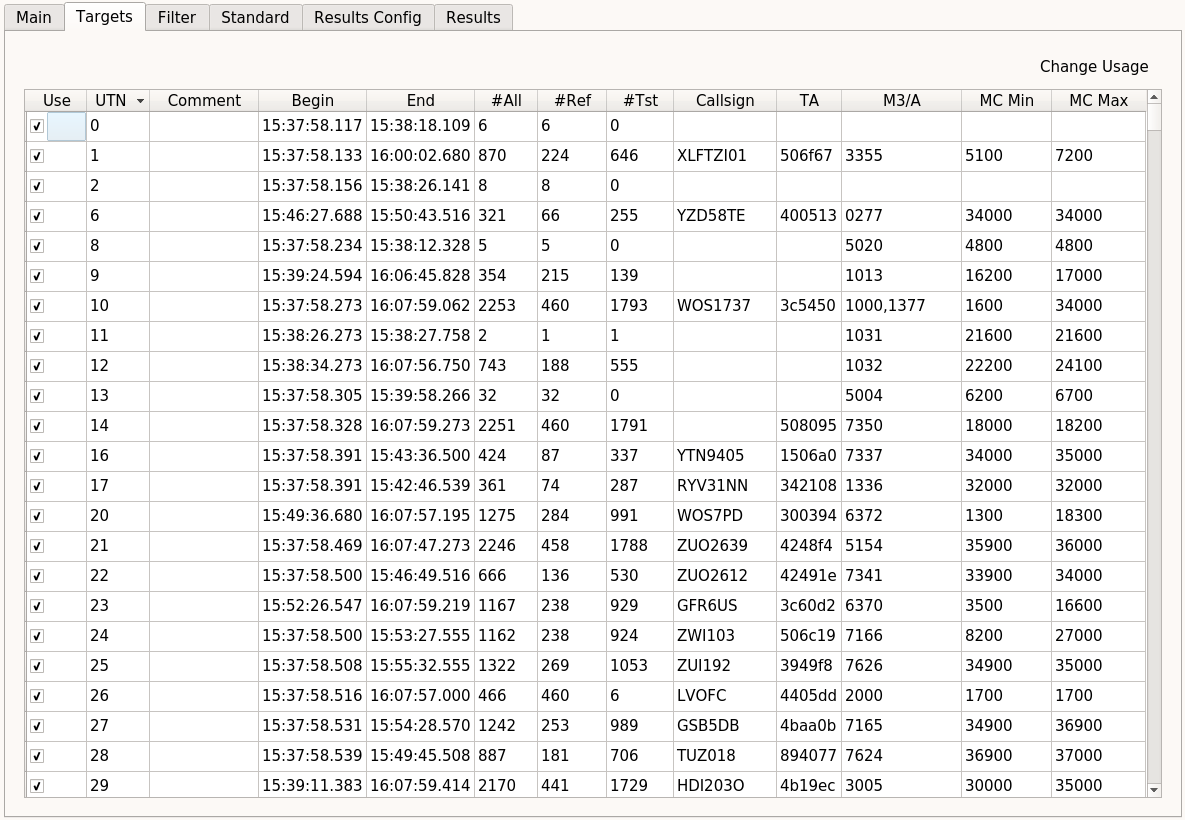
\includegraphics[width=18cm,frame]{figures/eval_targets_loaded.png}
  \caption{Evaluation Targets tab with loaded data}
\end{figure}



\subsection{Filter Tab}

\begin{figure}[H]
  \hspace*{-2cm}
    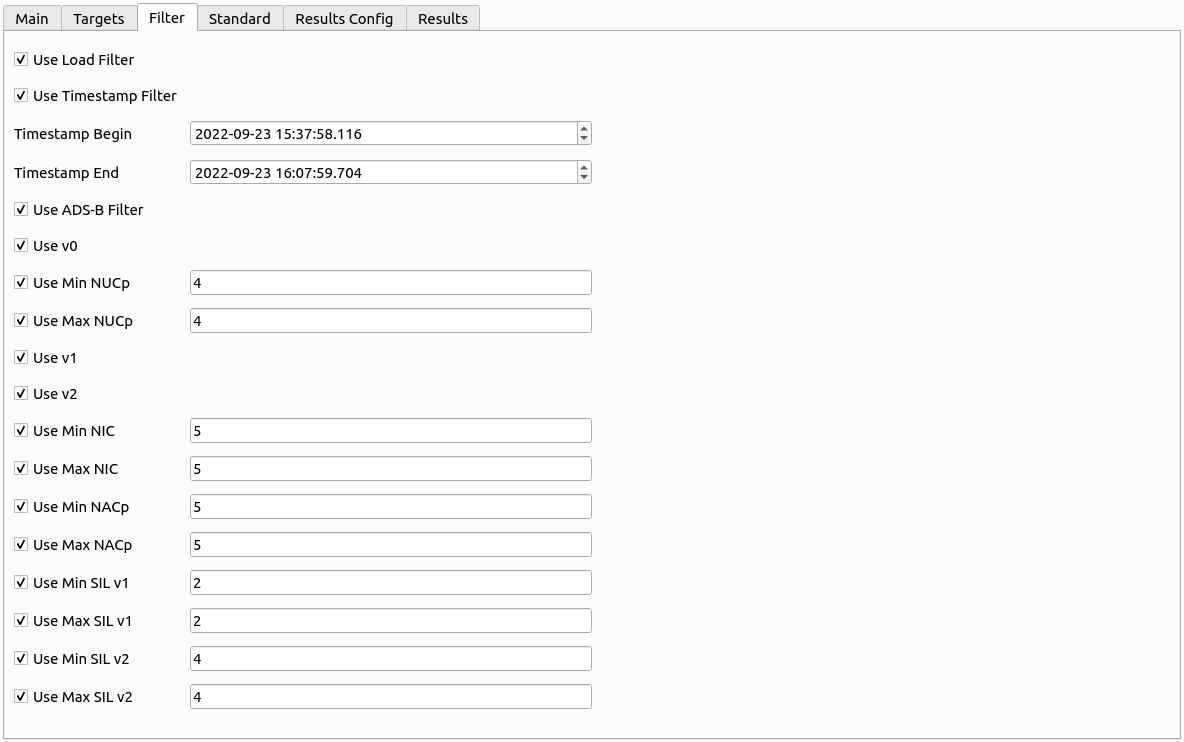
\includegraphics[width=18cm,frame]{figures/eval_filter.png}
  \caption{Evaluation Filter tab}
\end{figure}

In the Filter tab, what data is loaded for evaluation can be filtered \\

Below, the following elements exist:
\begin{itemize}  
\item 'Use Load Filter': Toggles usage of the load filter
\item 'Use Time Filter: Toggles usage of the time filter
\item 'Use ADS-B Filter: Toggles usage of the ADS-B filter
\item 'Use v0: Toggles usage of MOPS Version 0
\item 'Use Min NUCp: Toggles usage of the minimum NUCp value filter
\item 'Use Max NUCp: Toggles usage of the maximum NUCp value filter
\item 'Use v1: Toggles usage of MOPS Version 1
\item 'Use v2: Toggles usage of MOPS Version 2
\item 'Use Min NIC: Toggles usage of the minimum NIC value filter
\item 'Use Max NIC: Toggles usage of the maximum NIC value filter
\item 'Use Min NACp: Toggles usage of the minimum NACp value filter
\item 'Use Max NACp: Toggles usage of the maximum NACp value filter
\item 'Use Min SIL v1: Toggles usage of the minimum SIL v1 value filter
\item 'Use Max SIL v1: Toggles usage of the maximum SIL v1 value filter
\item 'Use Min SIL v2: Toggles usage of the minimum SIL v2 value filter
\item 'Use Max SIL v2: Toggles usage of the maximum SIL v2 value filter
\end{itemize}
\ \\

\subsection{Standard Tab}

\begin{figure}[H]
  \hspace*{-2cm}
    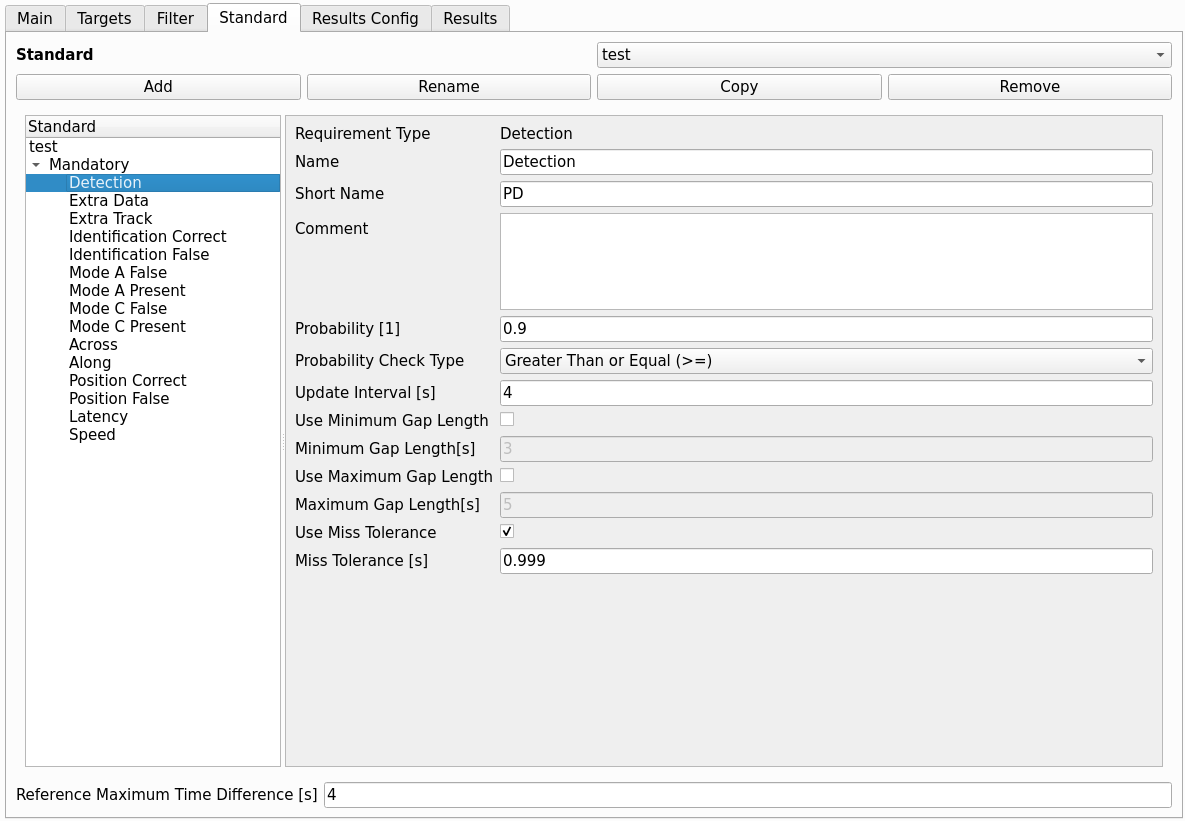
\includegraphics[width=18cm,frame]{figures/eval_standard.png}
  \caption{Evaluation Standard tab}
\end{figure}

In the Standard tab, at the top the current standard can be selected. \\

Below, the following buttons exist:
\begin{itemize}  
\item Add: Add a new standard with a unique name
\item Rename: Rename the current standard
\item Copy: Copy the current standart to a new one
\item Remove: Delete current standard
\end{itemize}
\ \\

At the bottom, the 'Reference Maximum Time Difference [s]' field can be edited to adjust the maximum time difference between reference updates. This value is used to find time-adjacent reference target reports for test target reports. Please adjust this value to e.g. the reference update peroid plus 1 second. \\

Currently, the following standards are (partly) supported:
\begin{itemize}  
\item EUROCAE ED-116 (\href{https://eshop.eurocae.net/eurocae-documents-and-reports/ed-116/}{Link})
\item EUROCAE ED-117/A (\href{https://eshop.eurocae.net/eurocae-documents-and-reports/ed-117a/}{Link})
\item EUROCAE ED-87C (\href{https://eshop.eurocae.net/eurocae-documents-and-reports/ed-87c/}{Link})
\end{itemize}
\ \\

Please note that, while the EUROCAE ED-117A has been tested using simulator data, the following limitations exist:
\begin{itemize}  
\item In the Stands area, the position accuracy should be calculated using a 5 second position averaging. This is currently not performed, since the averaging method is not specified, and is currently being discussed with users.
\item Some MLAT sensors use a different update rate for non-moving targets. This is currently not regarded, since what constituates non-movement is not (generally) specified, and will lower the probability of detection. 
\end{itemize}
\ \\

Please note that these limitations will be corrected in the near future. \\ 

The other standards have not yet been tested to the fullest degree, which is work in progress.


\subsubsection{Current Standard}

Below that, the current standard is shown. On the left side, a tree-view exists showing:
\begin{itemize}  
\item Standard name
\begin{itemize}  
\item Requirement Group(s)
\begin{itemize}  
\item Requirement(s)
\end{itemize}
\end{itemize}
\end{itemize}
\ \\

\begin{figure}[H]
  \hspace*{-2cm}
    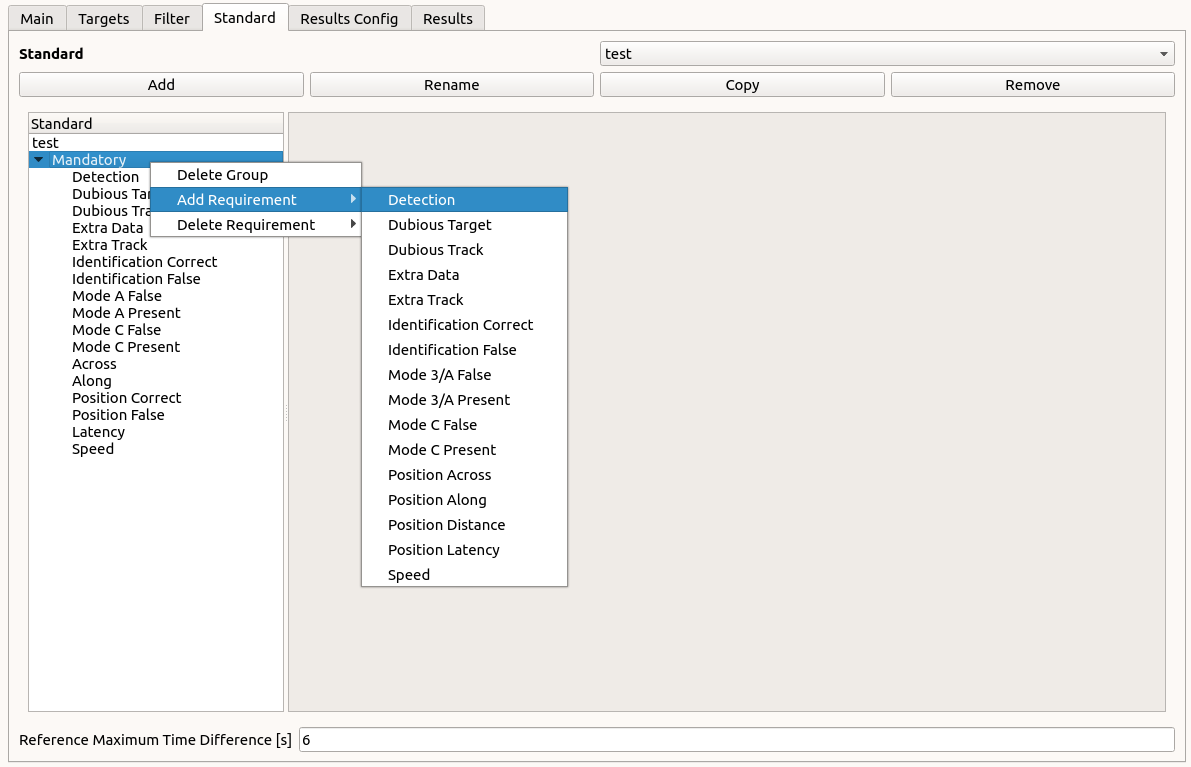
\includegraphics[width=18cm,frame]{figures/eval_standard_add_req.png}
  \caption{Evaluation Standard tab: Add requirement}
\end{figure}

When clicking on the standard name, a menu is shown allowing adding new requirement groups ('Add Group'). \\

When clicking on a requirement group, a menu is shown allowing the following functions:
\begin{itemize}  
\item Delete Group: Delete the selected requirement group
\item Add Requirement: Add a requirement of the selected type
\item Delete Requirement: Delete the selected requirement
\end{itemize}
\ \\

The following requirements exist:

\begin{center}
 \begin{table}[H]
  \begin{tabularx}{\textwidth}{ | l | X |  }
    \hline
    \textbf{Type} & \textbf{Description} \\ \hline
    \nameref{sec:eval_req_detection} & Calculates probability of detection  \\ \hline
    \nameref{sec:eval_req_extra_data} & Calculates probability of unused test data (test data w/o reference data) \\ \hline
    \nameref{sec:eval_req_extra_track} & Calculates probability of undetected tracks (reference data w/o test data) \\ \hline
    \nameref{sec:eval_req_id_correct} & Calculates probability of correct secondary identification \\ \hline
    \nameref{sec:eval_req_id_false} & Calculates probability of false secondary identification \\ \hline
    \nameref{sec:eval_req_m3a_false} & Calculates probability of false Mode 3/A code \\ \hline
    \nameref{sec:eval_req_m3a_present} & Calculates probability of Mode 3/A code present \\ \hline
    \nameref{sec:eval_req_mc_false} & Calculates probability of false Mode C code \\ \hline
    \nameref{sec:eval_req_mc_present} & Calculates probability of Mode C code present \\ \hline
    \nameref{sec:eval_req_pos_across} & Calculates the probability of the position across error begin within a threshold \\ \hline
    \nameref{sec:eval_req_pos_along} & Calculates the probability of the position along error begin within a threshold \\ \hline
    \nameref{sec:eval_req_pos_distance} & Calculates the probability of the position error begin within or outside a threshold \\ \hline
    \nameref{sec:eval_req_pos_latency}  & Calculates the probability of the position latency begin within a threshold \\ \hline
    \nameref{sec:eval_req_speed} & Calculates the probability of the speed error begin within or outside a threshold or percentage \\ \hline
\end{tabularx}
\end{table}
\end{center}
\ \\

If a requirement is clicked, it's configuration widget is shown on the right hand side. \\

Each requirement has the following common attributes:
\begin{itemize}  
\item Type: Type of the requirement
\item Name: Name of the requirement
\item Short Name: Abbreviated name of the requirement
\item Comment: Any text comment, e.g. reference to source document
\item Probability [1]: Probability threshold, as [0,1]
\item Probability Check Type: Probability comparison type for calculated probability against probability threshold
\end{itemize}
\ \\

For detailed information about each requirement please refer to section \nameref{sec:eval_requirements}.

\subsection{Results Tab}

\begin{figure}[H]
  \hspace*{-2cm}
    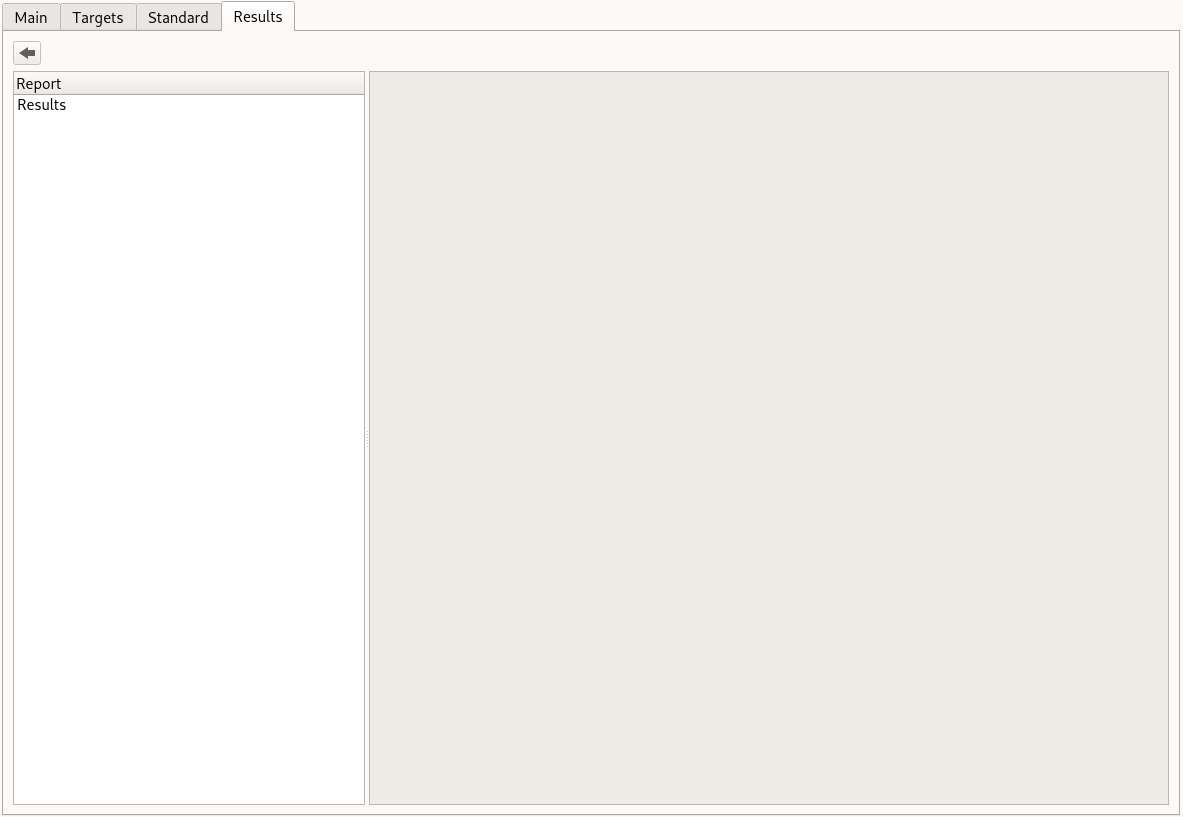
\includegraphics[width=18cm,frame]{figures/eval_results_empty.png}
  \caption{Evaluation Results tab}
\end{figure}

Before the data was evaluated, the results are empty.\\

There are several levels of detail for the results, and each sub-result is shown in a tree-view on the left side, grouped into sections. Using this tree-view, the results can be "navigated", and the currently selected results contents are shown on the right side. \\

More details will be described in the following section \nameref{sec:eval_inspect}.

\section{Running}
\label{sec:eval_run} 

\subsection{Load Data}
\label{sec:eval_run_load} 

After the wanted configuration (in the Main tab) has been set, the 'Load Data' button can be clicked. This results in the reference/test data being loaded, after which a post-processing will be performed. \\

Please note that the post-processing step uses all available cores on the CPU.

\begin{figure}[H]
  \centering 
    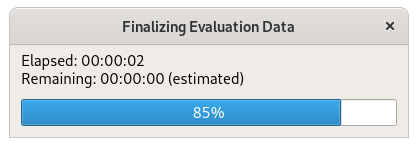
\includegraphics[width=8cm]{figures/eval_post.png}
  \caption{Evaluation: Post-processing after loading}
\end{figure}

The post-processing pre-calculates only which reference target reports can be used for direct comparison for specific test target reports. \\

Therefore, please note that re-loading the data is only required when changes to the reference/test data settings in the Main tab have been made. Changing requirements or removing targets from evaluation does not require re-loading. \\

After the loading and the post-processing have been performed, all targets are shown in the Targets tab.

\begin{figure}[H]
  \hspace*{-2cm}
    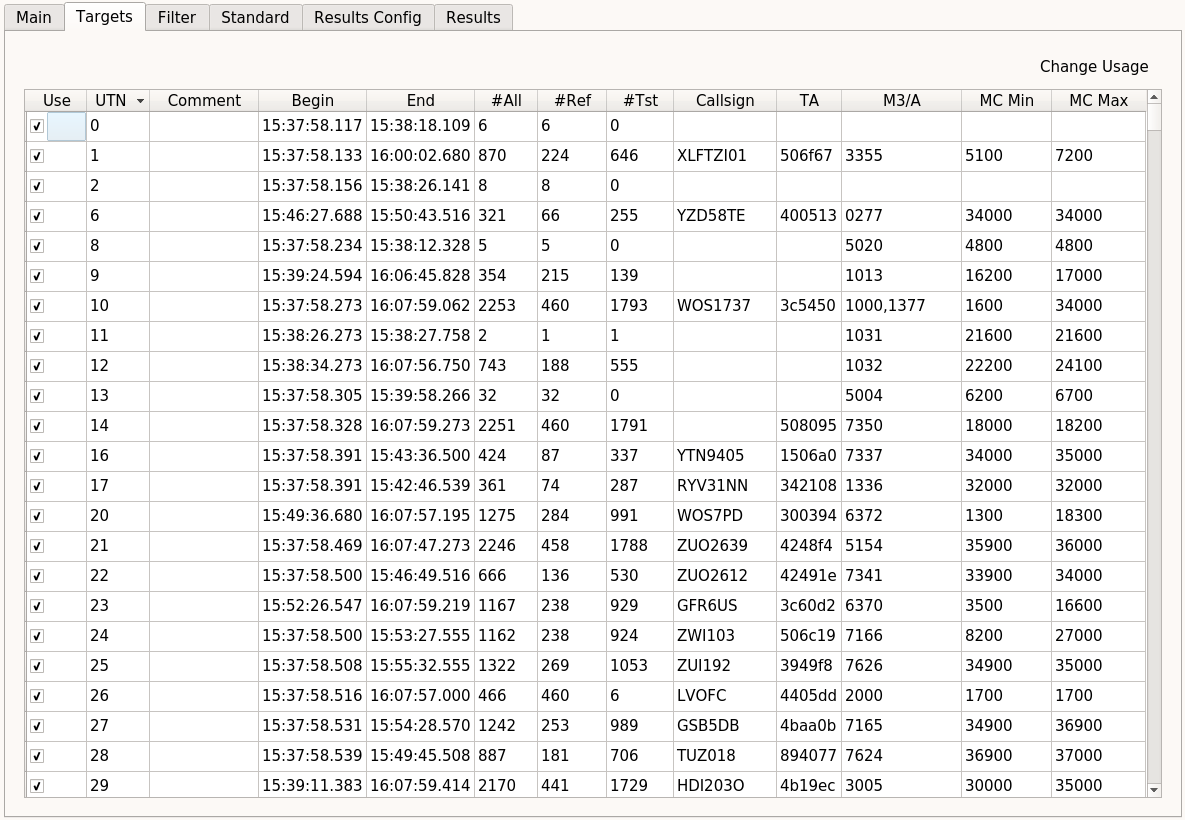
\includegraphics[width=18cm,frame]{figures/eval_targets_loaded.png}
  \caption{Evaluation Targets tab after loading}
\end{figure}

\subsection{Filtering Targets}
\label{sec:eval_filter_targets} 

The Targets tab is useful for removing certain targets from the evaluation ('Use' checkbox) and inspecting already removed ones. \\

Single rows can be selected by clicking on them, which triggers a loading process showing this exact target (with all associated data) in the available Views. Please note that this does not require re-loading the evaluation data, but can be used at all times during the evaluation. \\

The 'Change Usage' button can be used for the following actions:
\begin{itemize}  
\item Use All: Enable usage for all UTNs
\item Use None: Disable usage for all UTNs
\item Clear Comments: Clear comments of all UTNs
\item Filter: Start 'Filter UTNs' dialog
\end{itemize}
\ \\

The 'Filter UTNs' dialog can be used to dynamically filter UTNs based on the configurated values:

\begin{figure}[H]
    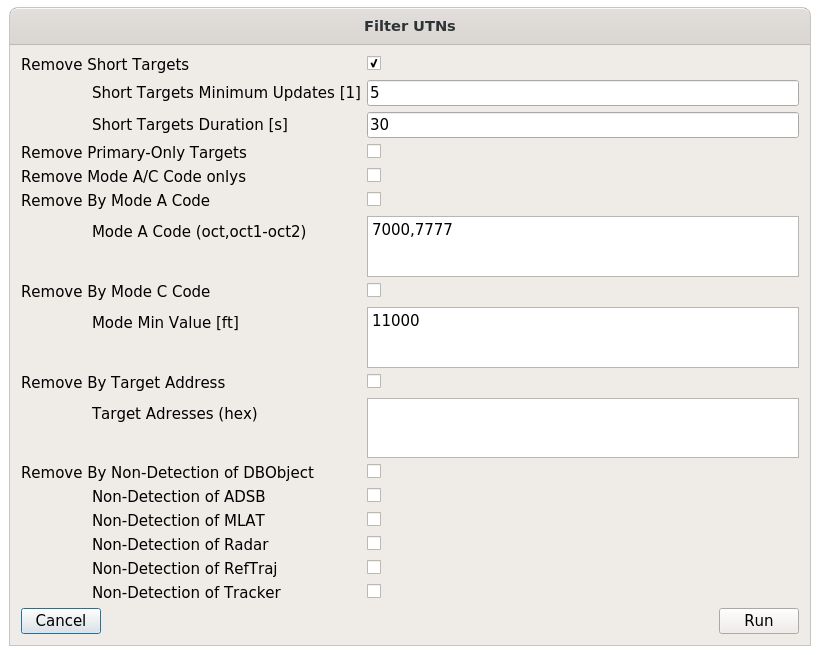
\includegraphics[width=15cm]{figures/eval_filter_utns.png}
  \caption{Evaluation Filter UTNs dialog}
\end{figure}

\begin{itemize}  
\item Remove Short Targets: Removes targets with a small number of target reports or duration
\item Remove Primary-Only Targets: Removes primary-only targets (w/o secondary attributes)
\item Remove Mode A/C Code onlys: Removes targets without Mode S attributes
\item Remove by Mode A Code: Removes targets having a Mode A code given in the list
\item Remove by Mode C Code: Removes targets having a Mode C code smaller than the given value
\item Remove by Target Address: Removes targets having a Mode S target address given in the list
\item Remove by Non-Detection of DBObject: Removes targets not being detected by a given DBOObject (e.g. sensor type)
\end{itemize}
\ \\

When the 'Run' button is clicked, all (enabled) targets are checked and are disabled if any of the selected filters apply.

\begin{figure}[H]
  \hspace*{-2cm}
    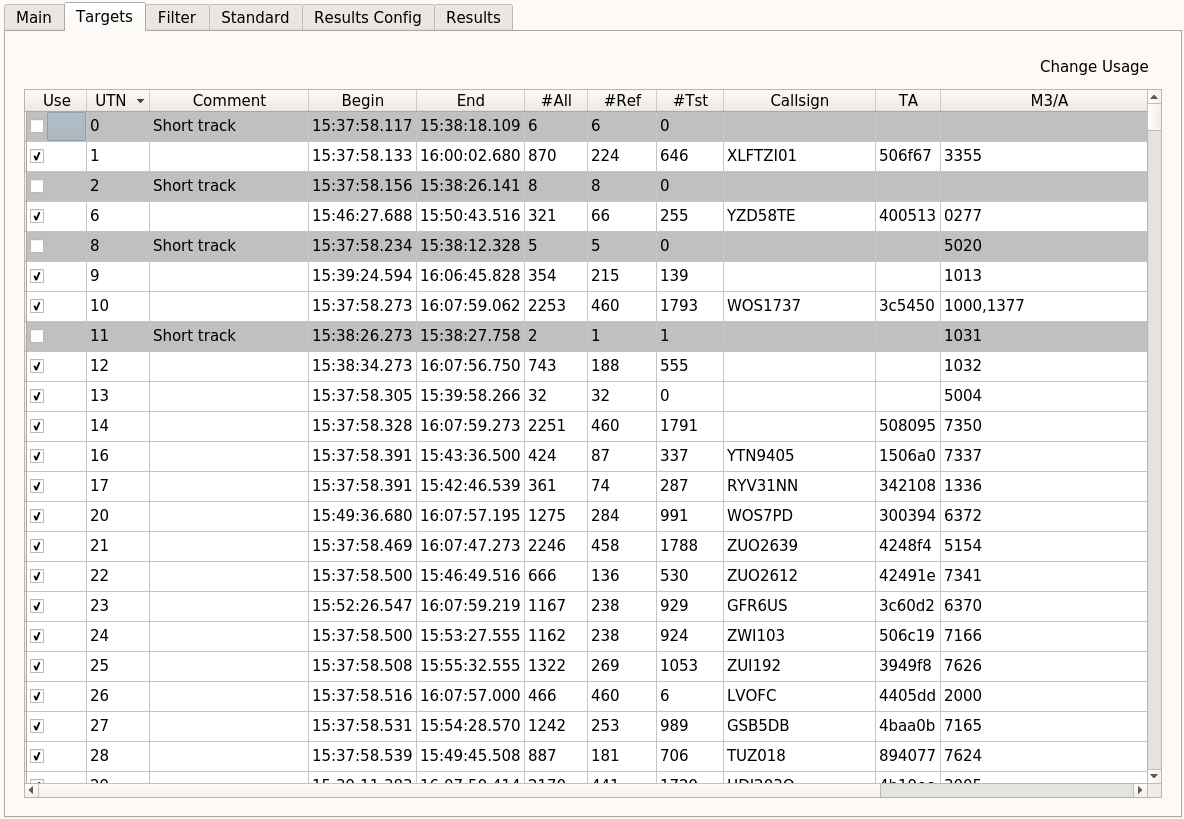
\includegraphics[width=18cm,frame]{figures/eval_targets_filtered.png}
  \caption{Evaluation Targets tab after filtering}
\end{figure}

Please note that the 'Change Usage' button can be used also after the 'Evaluate' button is used, which automatically updates the evaluation results.

\subsection{Evaluation}
\label{sec:eval_run_eval} 

After the data was loaded, the configuration relating to current standard, requirements and sector/requirement group usage can be adapted. After that, the evaluation can be (re-)run using the 'Evaluate' button. \\

This will trigger evaluation of the requirements in all sectors (as configured). The requirement values will be calculated for each target (whether to be used or not). Then, for each requirement and sector, the results are summed-up as per-sector average (if target should be used). \\

Please note that the post-processing step uses all available cores on the CPU.

\begin{figure}[H]
  \centering 
    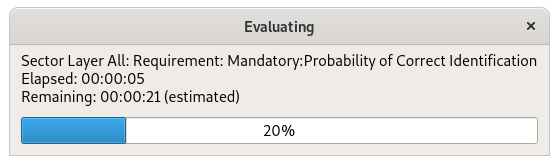
\includegraphics[width=10cm]{figures/eval_eval_status.png}
  \caption{Evaluation: Running evaluation status}
\end{figure}

The results are then shown in the Results tab.

\section{Results Inspection \& Analysis}
\label{sec:eval_inspect}

As described before, there are several levels of detail in which sub-results can be inspected.\\

The uppermost is the 'Requirements$\rightarrow$Overview', giving the sector sums for all requirements. \\

The next level of detail are the sector sum details, located in 'Sectors$\rightarrow$Sector Layer Name$\rightarrow$Requirement Group Name$\rightarrow$Requirement Name'. \\

The lowest level are the per-target details, located in 'Targets$\rightarrow$UTN' and the respective per-target results located in 'Targets$\rightarrow$UTN$\rightarrow$Sector Layer Name$\rightarrow$Requirement Group Name$\rightarrow$Requirement Name'. \\

By default, when single-clicking a row in a table the respective results are shown in the existing Views. When double-clicking, a step into the next level of detail is performed (if available). \\

Navigation can be made more efficient by returning to the last sub-result by using the 'Back' button on the top-left.

\subsection{Overview}
\begin{figure}[H]
  \hspace*{-2cm}
    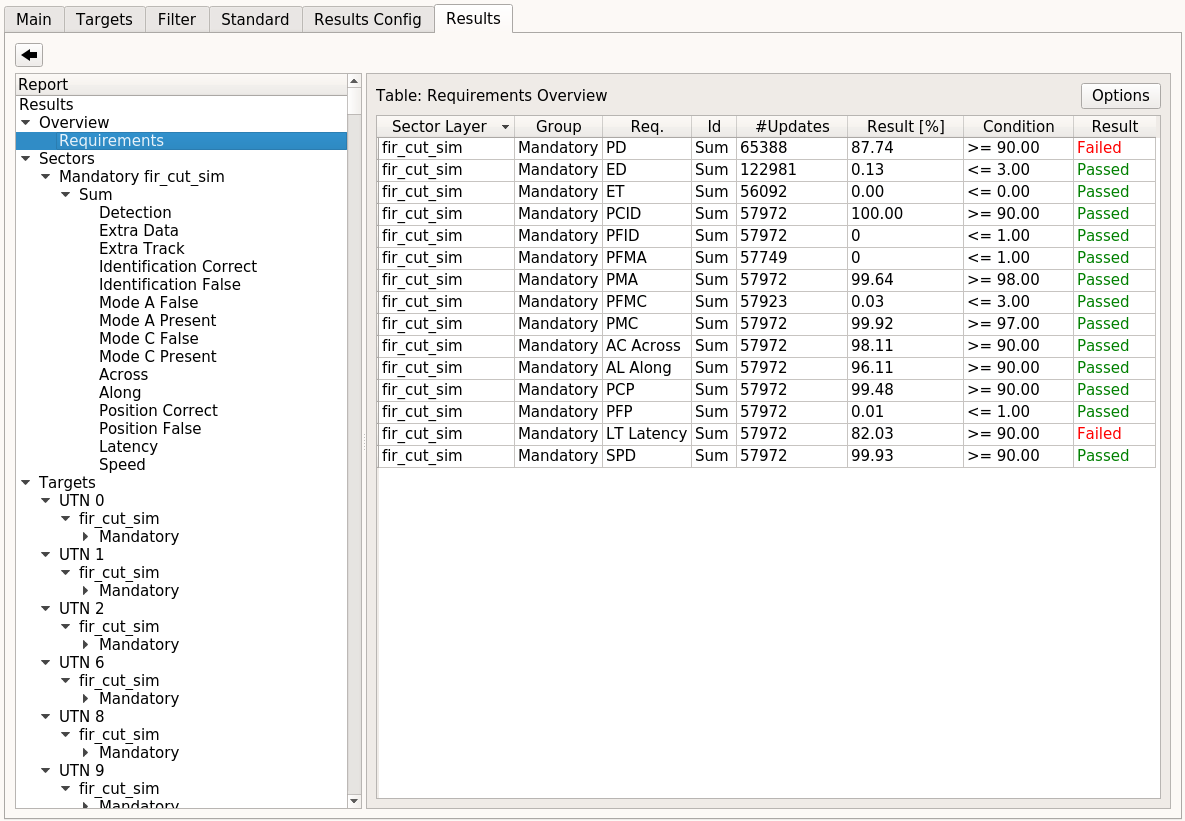
\includegraphics[width=18cm,frame]{figures/eval_results_overview.png}
  \caption{Evaluation results: Overview}
\end{figure}

Please note that the results are given as example only and are no indication of performance for any system currently in operation. \\

When single-clicking a row, the respective result error are shown in the existing Views.

\begin{figure}[H]
  \hspace*{-2.5cm}
    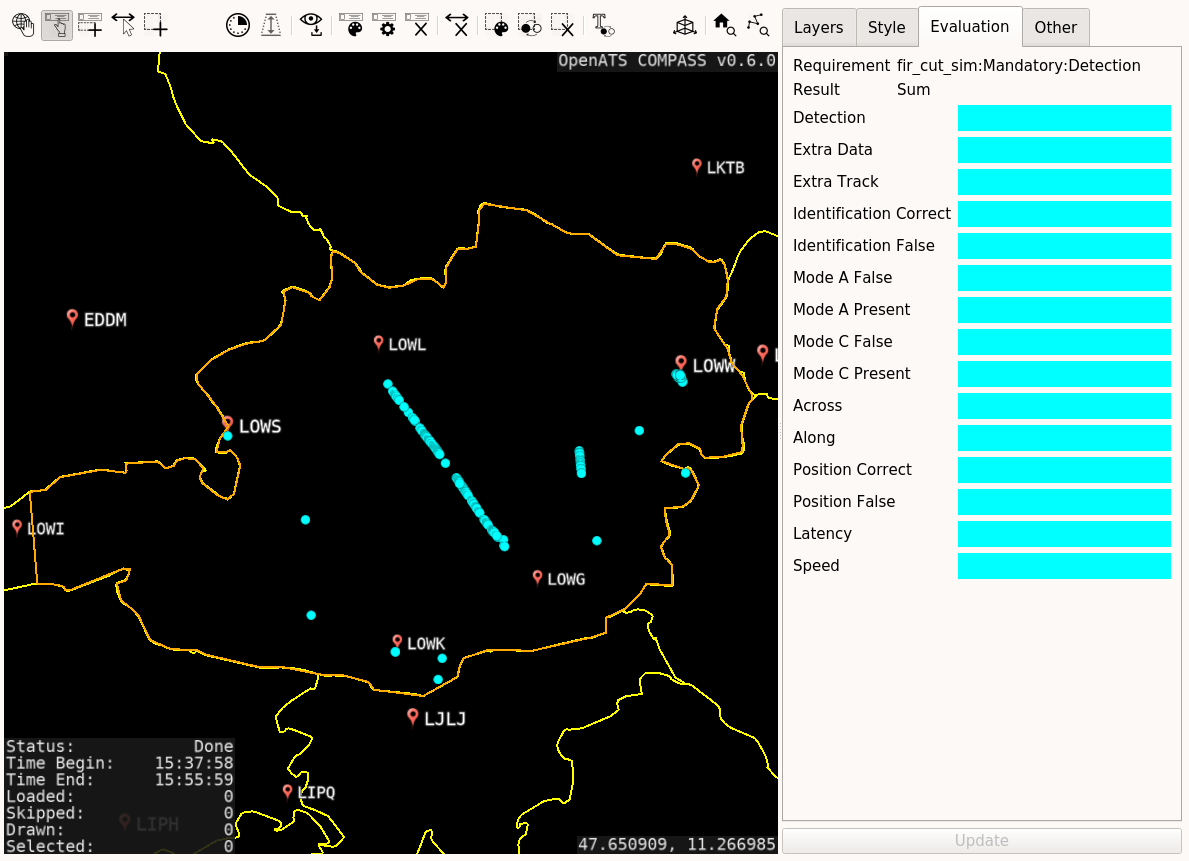
\includegraphics[width=19cm,frame]{figures/eval_results_pd_sum_osgview.png}
  \caption{Evaluation results: Sector PD errors in OSGView}
\end{figure}

When double-clicking a row, a step into the respective sector sum details is performed.

\subsection{Sector Details}

\begin{figure}[H]
  \hspace*{-2cm}
    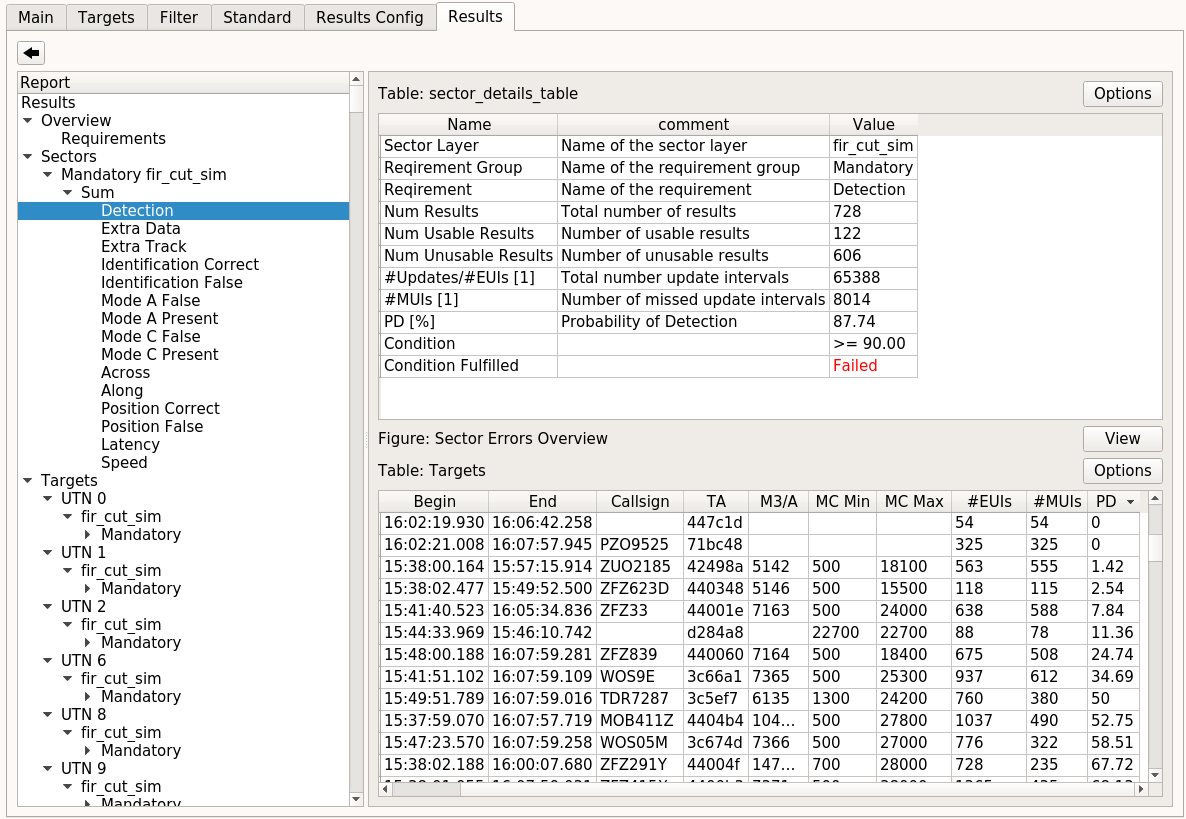
\includegraphics[width=18cm,frame]{figures/eval_results_sec_det_example.png}
  \caption{Evaluation results: Sector Detail Example}
\end{figure}

On the left side, the current position in the results sections is shown. On the right, the current results are shown. At the top, there is an overview table giving the details of the calculation results in the respective sector layer and requirement. \\

At the bottom, further result details are listed per-target, sorted in this example by the Probability of Detection (PD). \\

When single-clicking a row, the respective target data and result errors are shown in the existing OSGViews.

\begin{figure}[H]
  \hspace*{-2.5cm}
    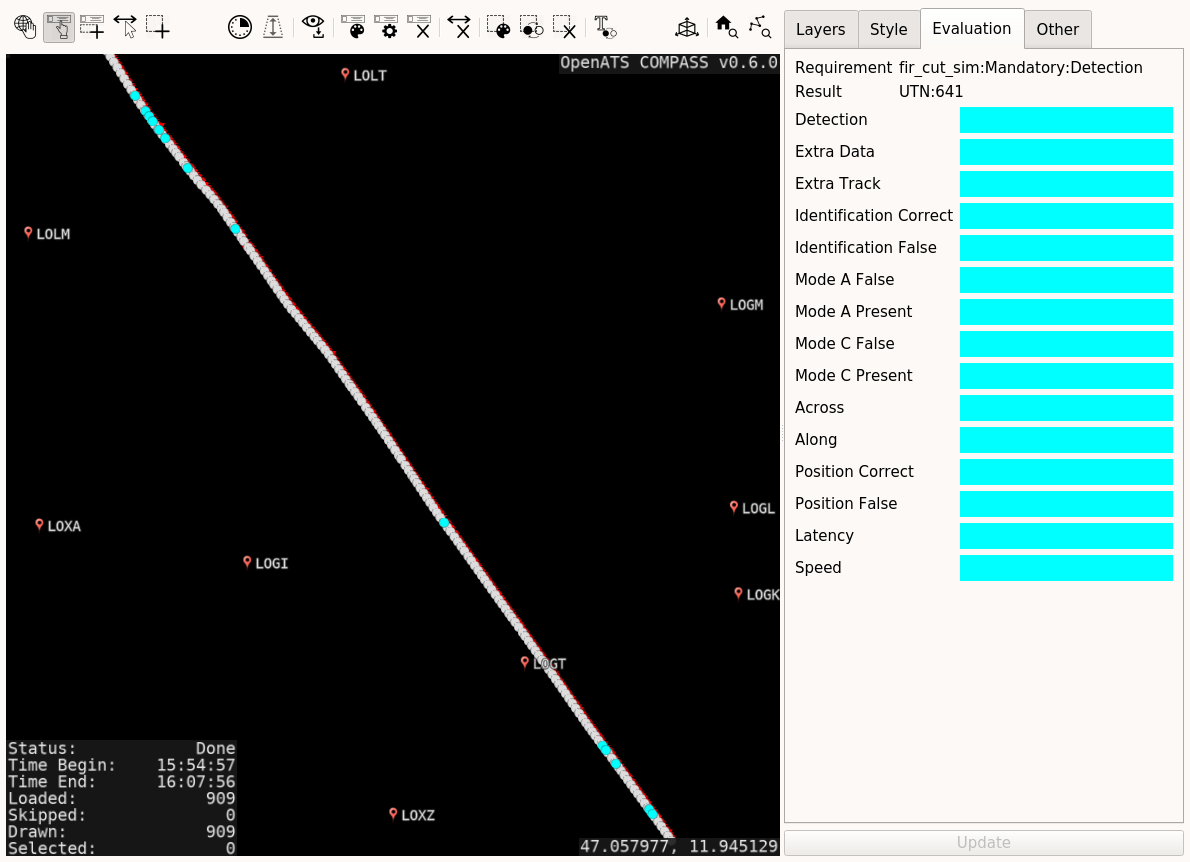
\includegraphics[width=18cm,frame]{figures/eval_results_pd_single_osgview.png}
  \caption{Evaluation results: Target PD Errors in OSGView}
\end{figure}

When double-clicking a row, a step into the respective target details is performed.

\subsection{Per-Target Details}

\begin{figure}[H]
  \hspace*{-2cm}
    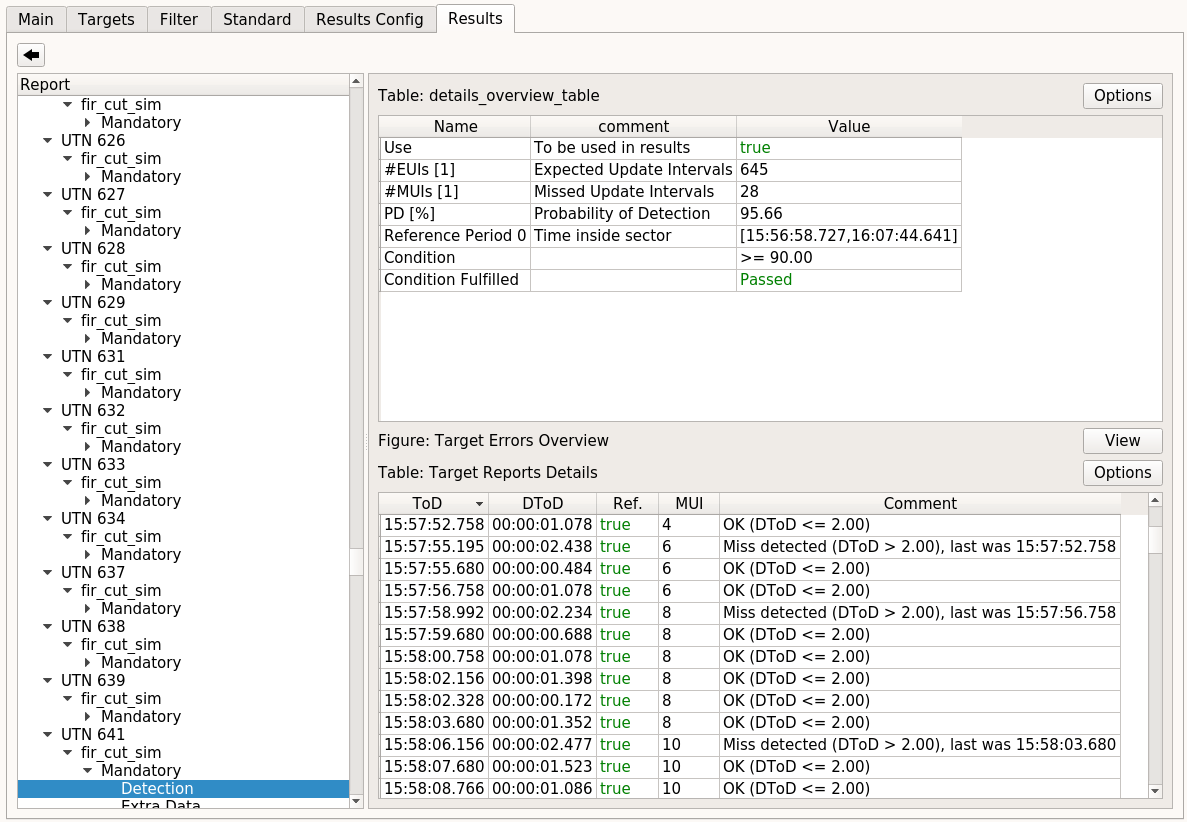
\includegraphics[width=18cm,frame]{figures/eval_results_target_det_example.png}
  \caption{Evaluation results: Per-Target PD Detail Example}
\end{figure}

On the left side, the current position in the results sections is shown. On the right, the current results are shown. At the top, there is an overview table giving the details of the calculation results for the target in the respective sector layer and requirement. \\

At the bottom, further result details are listed per-target-report, sorted in this example by time. \\

When single-clicking a row, the respective target data and the respective single result error are shown in the existing OSGViews.

\begin{figure}[H]
  \hspace*{-2.5cm}
    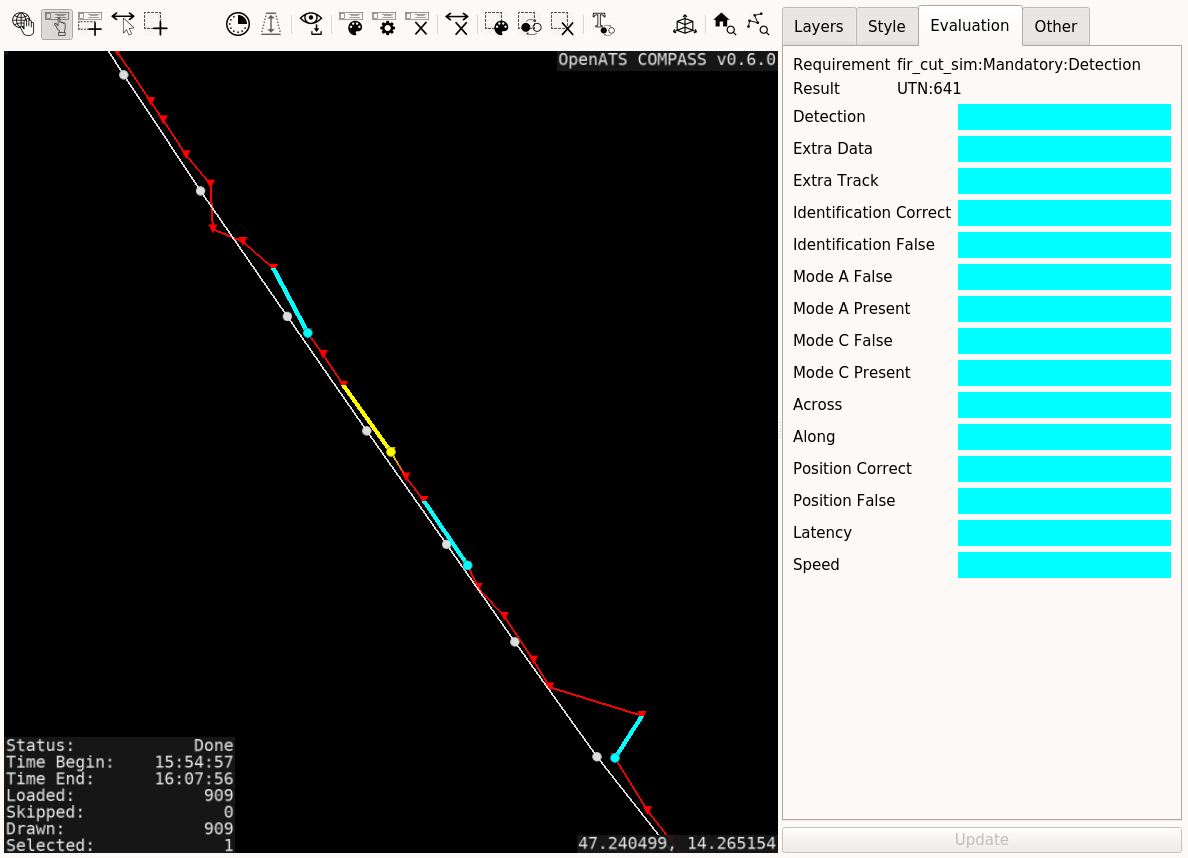
\includegraphics[width=19cm]{figures/eval_results_pd_single_tr_osgview.png}
  \caption{Evaluation results: Target Single PD Error in OSGView}
\end{figure}


\section{Generate Report}
\label{sec:eval_report}

Using the "Export PDF" button, a PDF can be generated.

\begin{figure}[H]
    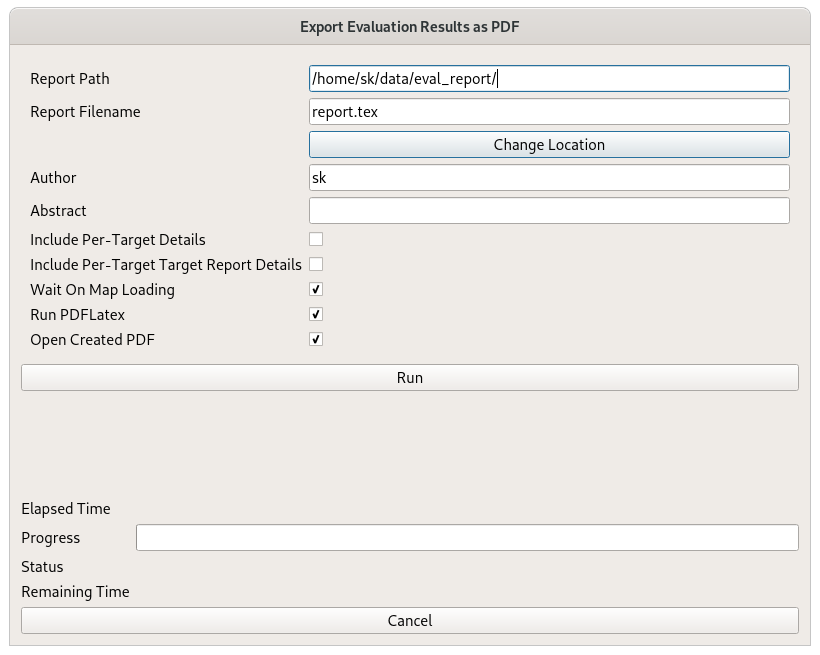
\includegraphics[width=14cm]{figures/eval_report.png}
  \caption{Evaluation results: Generate report dialog}
\end{figure}

At the top, the following configuration options exist:

\begin{itemize}  
\item Report Path: Directory to which the report will be written.
\item Report Filename: Filename of the report, to be created in the report path. File extension must be '.tex'.
\item Change Location: Button to set the report path and filename.
\item Author: Author string, is added to the first page of the report.
\item Abstract: Abstract string, is added to the first page of the report.
\item Include Per-Target Details: Whether to include the per-target details.
\item Include Per-Target Target Report Details: Whether to include the per-target target report details.
\item Wait on Map Loading: When OSGView screenshots are created, some maps require downloading terrain from the Internet.  This option enables to wait on completion of such activities, to generate high-quality screenshots. Disable only when operating on cached maps without an Internet connection.
\item Run PDFLatex: Automatically runs the pdflatex compile process, immediately creating a PDF after finished export. Is disabled if command could not be found.
\item Open Created PDF: Automatically opens the created PDF. Is disabled if pdflatex command could not be found.
\end{itemize}
\ \\

Please \textbf{note} that the two 'Include ... Details' options can produce very large PDF reports (10.000+ pages), and may even overload the Latex sub-system (will result in 'TeX capacity exceeded, sorry' error). It is therefore recommended to only activate these options for small datasets with very few sector layers. \\

The 'Run' button startes the export process. At the bottom, status information and a cancel button exists. \\

To run the export process, click the 'Run' button.

\begin{figure}[H]
    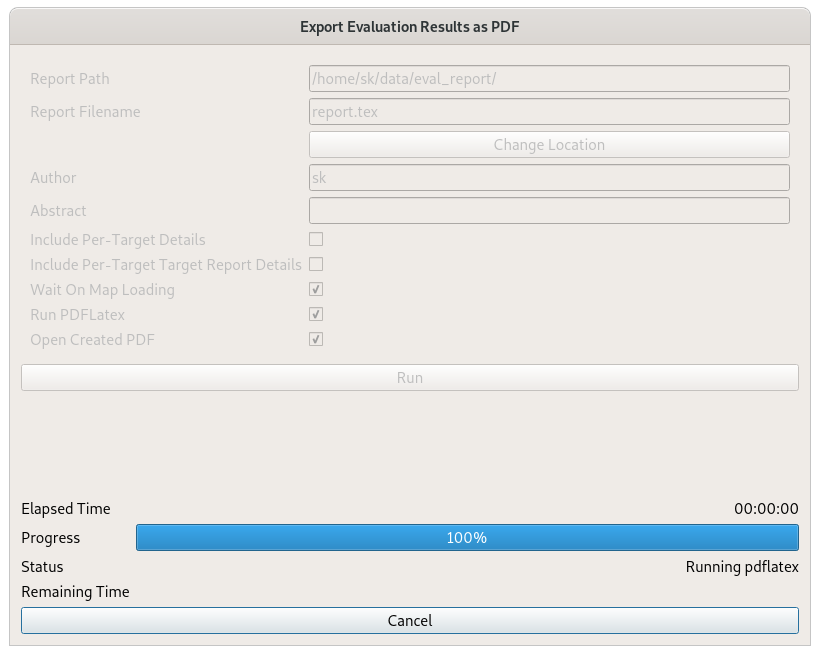
\includegraphics[width=14cm]{figures/eval_report_status.png}
  \caption{Evaluation results: Generate report in progress}
\end{figure}

If the export process was sucessful, the dialog is closed automatically. The report Latex file was written into the report directory, with screenshots in the 'screenshots' subfolder. If the respective options were set, a PDF was automatically generated and is opened using the default PDF application. \\

If a Latex error ocurred, a message box with the error message is shown. If the 'TeX capacity exceeded, sorry' error is shown, disable one or both of the 'Include ... Details' options.\\

Please note that the generated report can of course be edited by the user and re-generated using pdflatex, which allows for better customization options (adding e.g. details, corporate identity etc.).

\subfile{eval_requirements}
